\chapter{Literature} \label{ch:literature}

\section{Introduction}
Hardware developments in the last two decades (2000-2020) have enabled deep-learning algorithms to achieve state-of-the-art image segmentation in the field of computer vision, outperforming humans on many classification tasks \cite{ioffe2015, He2015, Wu2015}. The following review aims to cover recent developments in medical image segmentation by focusing on network architecture, training methods, and challenges in the context of radiotherapy (RT). We begin by examining variability in the definition of organs contoured by medical professionals, and outline a novel technique used by Nikolov et al. that takes this variability into account when assessing model performance \cite{Nikolov_2018}. Further, we explain U-Net architecture in detail before expanding on the original work by examining modifications in recent implementations. We conclude the review by outlining class imbalance as an optimisation challenge in segmentation.


\section{Observer variability in contour delineation}
 
Uncertainty in the delineation of contour volumes is a significant source of error in radiotherapy (RT) \cite{Nikolov_2018}. Multiple studies have highlighted accurate contouring as a requirement for effective clinical outcomes \cite{Vinod_2016, Roach_2019, Nemoto_2020}, and note that current inter and intra-observer variability creates a challenge for quality assurance (QA) of dosimetric impact \cite{Vinod_2016}. Additionally, inconsistencies in adherence to contouring protocols have the potential to introduce variability when cross-referencing the results of clinical trials \cite{Roach_2019}. Investigations into the contouring quality of trials have revealed that up to 80\% of audited files would require modification for protocol compliance \cite{Kachnic2013}. A separate study found a 25\% non-compliance rate in a phase 3 trial for head and neck RT - primarily due to incorrect target contouring - which was associated with a 20\% decrease in 2-year survival rates \cite{Peters2010}. High-quality contours are often achieved through a combination of highly skilled multidisciplinary teams, taking into account additional data beyond patient imaging \cite{Vinod_2016, Roach_2019}. However, in attempts to decrease variability and its impact on treatment outcomes, studies report the benefit of automatic contouring tools as a starting reference (when available) \cite{Vinod_2016}, and highlight the need for volume delineation to become part of routine QA \cite{Vinod_2016}. 

While automatic contouring has been shown to improve consistency in delineation \cite{Vinod_2016}, current commercial solutions do not provide a fully automated experience \cite{Nemoto_2020}. For instance, Varian Medical Systems `Smart Segmentation' tool includes the trachea and main bronchi in normal lung delineations, contrary to the RTOG 1106 guideline for lung cancer RT \cite{Nemoto_2020}. Hence, there is a need for alternative contouring tools in RT that provide more accurate delineation \cite{Nemoto_2020}, and feedback on the accuracy of manual corrections for QA \cite{Nikolov_2018}.

In RT, IOV is often larger than errors associated with patient setup and organ motion \cite{Vinod_2016, Murakami2013}; however, the extent is also organ dependent \cite{Roach_2019}. A 2019 study measured IOV on diagnostic computed tomography (CT) for prostate cancer treatment and found ``excellent agreement'' for bladder, rectum, and clinical target volume contours (defined by an inter-observer variability assessment (ICC) value $>$ 0.75), and reported the extent of variation to serve as a benchmark for comparison \cite{Roach_2019}.  A total of 5 patients were included in the study, selected to represent the broad range of anatomy within clinical trials. Contouring was performed by 13  observers (9 radiation oncologists) across multiple clinic locations, with guideline examples distributed to all observers before study commencement. Bladder volume agreement was measured to be 0.93 $\pm$ 0.03 via the dice similarity coefficient (DSC \cite{Dice1945} - see equation \ref{eq:DSC} and Figure \ref{fig:sDSC}), with absolute mean surface distance (MSD) ranging from 0.76 mm to 1.44 mm across patients \cite{Roach_2019}. DSC agreement for the rectum was  0.81 $\pm$ 0.07, and a MSD of 1.97mm to 4.14mm \cite{Roach_2019}. Although variance for the rectum was higher than that of the bladder, external studies report that a DSC $\geq$ 0.7 is considered clinically acceptable for these organs \cite{Roach_2019, Sharp2014}. Duc et al. note that a high DSC value should guarantee clinical acceptability in RT - but do not define `high' \cite{Duc}. Consistent IOV is reported across the literature for male bladder and rectum contouring via diagnostic CT \cite{Riegal2016}.

Although a high DSC should guarantee clinical acceptability, a lower DSC does not necessarily mean that an automatic segmentation is not clinically useful.

\section{Defining an expert performance metric for model evaluation}
Although automated segmentation tools are in clinical use \cite{Zhu_2018}, current performance tends to be poor when compared to expert delineation - especially in the case of small organ segmentation \cite{Nikolov_2018, Zhu_2018}. Consequentially, they are typically used as a starting reference and require time-consuming corrections \cite{Nikolov_2018, Nemoto_2020}. A study developed by Google's DeepMind highlights an additional barrier to deep-learning solutions (which have shown significant improvements in accuracy and inference time over traditional methods \cite{Zhu_2018}) is the absence of a clinically-relevant metric that takes into account expert IOV when assessing model performance \cite{Nikolov_2018}. The study suggests that the typical DSC metric is a poor measure of similarity between model and expert if operating under the assumption that manual correction is required \cite{Nikolov_2018}. DSC is a commonly used volumetric overlap score (equation \ref{eq:DSC}) in medical image segmentation \cite{Taha_2015}. However, DSC does not penalise a model for the number of contour surface points that must be manually adjusted \cite{Nikolov_2018} - which may be an important indicator of time required for correction \cite{Nikolov_2018}. In an attempt to overcome these limitations, Nikolov et al. introduced a novel surface dice similarity metric (sDSC), which measures the similarity between two contour boundaries and normalises to be independent of organ volume. This metric defines expert performance $\tau$ as the 95th percentile MSD between observers (specific to each organ considered) and enforces no penalty when surface deviations are within this tolerance \cite{Nikolov_2018}. In contrast to the DSC metric,  sDSC measures the proportion of surfaces in a contour set which are within expert IOV; providing direct information on the degree of manual correction required \cite{Nikolov_2018}. Successful model performance was defined by Nikolov et al. as a cross-patient average sDSC $\geq$ 95\%. An illustration of the proposed metric is included in Figure \ref{fig:sDSC},
where $M_{i}$ represents the volumetric mask considered in DSC measures, $B_{i}^{(\tau)}$ represents the contour surface $S_{i}$ with IOV tolerance $\tau$, and $S_{i} \cap B_{j}^{(\tau)}$ is the intersection of surface boundaries at an organ-specific tolerance $\tau$. The sDSC metric is stated in equation \ref{eq:sDSC} \cite{Nemoto_2020}, while the standard DSC is included for comparison in equation \ref{eq:DSC} \cite{Bertels2019}.

\begin{equation}
sDSC_{i,j}^{(\tau)} = \frac{|S_{i} \cap B_{j}^{(\tau)}| + |S_{j} \cap B_{i}^{(\tau)}|}{|S_{i}| + |S_{j}|}
\label{eq:sDSC}
\end{equation}

\begin{equation}
DSC_{i,j} = \frac{2|M_{i} \cap M_{j}|}{|M_{i}| + |M_{j}|}
\label{eq:DSC}
\end{equation}

However, the proposed metric has yet to see clinical implementation. As such, Nikolov et al. recommend reporting sDSC values alongside typical DSC measures to compare performance across the literature \cite{Nikolov_2018}. An additional limitation in the use of sDSC (a so-called `hard' metric) is the introduction of a disharmony between model optimisation and target performance \cite{Bertels2019}. Hard metrics assume binary segmentation as input; therefore, soft surrogates (accepting continuous data) are required to define differentials for gradient descent algorithms \cite{Bertels2019}. Recent studies have proposed soft DSC as a loss function that can directly optimise the DSC performance metric \cite{Bertels2019}; however, no such surrogate currently exists for the sDSC due to difficulties in defining surface integrals on boundaries represented by continuous segmentation values. Multiple sources in the literature have highlighted the benefit of directly optimising for the metric used to evaluate model performance \cite{Bertels2019, Vapnik2000}.

\begin{figure}
	\begin{center}
		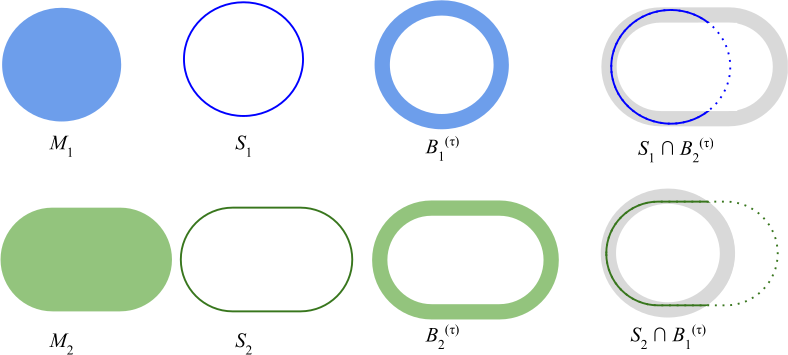
\includegraphics[width=0.85\textwidth]{sDSC}
		\caption{Illustration of equation variables seen in DeepMind's proposed surface dice similarity coefficient (sDSC), equation \ref{eq:sDSC}; and typical dice similarity coefficient (DSC), equation \ref{eq:DSC} for contours i, j. $M_{i}$ represents the volumetric mask considered in DSC measures, $B_{i}^{(\tau)}$ represents the contour surface $S_{i}$ with inter-observer variance (IOV) tolerance $\tau$, and $S_{i} \cap B_{j}^{(\tau)}$ is the intersection of surface boundaries at organ specific tolerance $\tau$: defined as the $95^{th}$ percentile absolute mean surface distance (MSD) between expert observer contours, specific to each organ considered. Figure redrawn from Nikolov et al. \cite{Nikolov_2018}.}
		\label{fig:sDSC}
	\end{center}
\end{figure}

Vaassen et al. attempted to measure the relationship between the sDSC and time required for contour correction \cite{vaassen2020}, as seen in Figure \ref{fig:vaassen}. However, this study failed to use a 95th percentile MSD for each organ-specific tolerance, as described by Nikolov et al. Rather, a value of 1 mm was used for all organs at risk (OARs), corresponding to the x-y pixel resolution used in the study's CT scans \cite{vaassen2020}. Hence, sDSC values presented in this study are representative of variance due to spatial resolution limits and not IOV. MSD$_{95}$ values calculated from Roach et al. show organ-specific tolerances of 1.46 mm for the bladder, and 6.99 mm for the rectum. Thus, we expect sDSC values reported by Vaassen et al. to be significantly lower \cite{Nikolov_2018}, and have poorer predictive validity than when considered under correct IOV assumptions. Despite this limitation, the sDSC was a significantly better indicator of time required for correction when compared to the DSC and mean Hausdorff distance (MSHD) metrics \cite{vaassen2020}.
A query of all PubMed articles referencing surface dice similarity since Nikolov et al. found no other attempts to correlate sDSC with correction time.

\begin{figure}[H]
	\begin{center}
		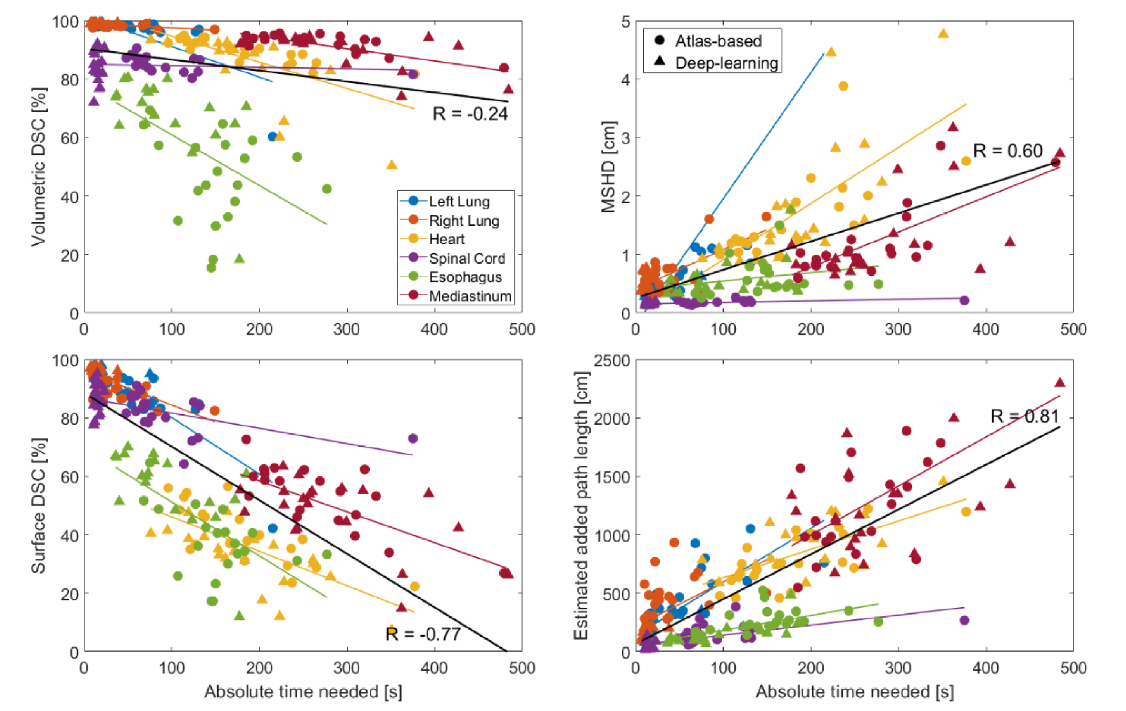
\includegraphics[width=1\textwidth]{vaassen_large}
		\caption{Vaassen et al. compare common segmentation similarity metrics with surface DSC (sDSC \cite{Nikolov_2018}) and their novel `estimated added path length' metric for ability to infer absolute time required for automatic contour correction. Atlas-based (circles) and deep-learning (triangles) methods combined. Correlation coefficients indicate a stronger relationship between sDSC value and time required, than dice similarity coefficient (DSC) and mean Hausdorff distance (MSHD) \cite{Vaassen_2020}. We note a limitation to this study is the use of an incorrect organ specific tolerance (1.0 mm - voxel size), compared to the organ specific inter-observer variance tolerance $\tau$ defined in Nikolov et al. \cite{Nikolov_2018}. Figure redrawn from Vaassen et al.  \cite{Vaassen_2020}.}
		\label{fig:vaassen}
	\end{center}
\end{figure}



\section{Historical U-Net architecture}
A 2015 study by Ronneberger et al. expanded on the concept of fully convolutional networks (FCNs by Long et al. \cite{Long2014}) to meet the challenges posed by a lack of curated training data for biomedical image segmentation \cite{Ronneberger_2015}; and to tailor FCNs for pixel-wise classification (semantic segmentation) \cite{DLINMI2018}. This breakthrough `U-Net' architecture (Figure \ref{fig:unet}) includes a contracting pathway (typical of past FCNs) which downsamples resolution in the image plane to capture contextual (high-level) features for detection and general localisation \cite{Nemoto_2020}; as well as an expanding pathway, whereby high-resolution feature maps are  concatenated with matching upsampling blocks via residual skip connections \cite{Maier2019} to recover full spatial resolution in the model output \cite{DLINMI2018}. Studies report concatenating high-resolution feature maps via this secondary path improves local (detailed) feature propagation \cite{Nemoto_2020}, as later convolutions operate over both the high-resolution information provided by skip connections, and the contextual features passed via upsampling. Hence, U-Net architecture facilitates multi-resolution analysis \cite{Maier2019} in an attempt to overcome the trade-off between local feature propagation and the use of contextual information in segmentation \cite{Hesamian2019}. For instance, larger kernel sizes relative to the input resolution infer spatially broader information; although, require additional pooling layers, decreasing local accuracy for detailed segmentation borders \cite{Hesamian2019}. However, studies have indicated that this trade-off still exists, as shallow U-Net models tend to perform better on small segmentation regions \cite{Zhu_2018}.

Contracting (encoding) blocks were composed of two convolutional layers with 3 x 3 kernel sizing, doubling the feature channels of the input before downsampling the x-y resolution via 2 x 2 max-pooling \cite{Ronneberger_2015}. External studies have demonstrated the importance of increasing channels before max-pooling operations to avoid computational bottlenecks \cite{szegedy2015}; a strategy adopted in both paths of typical U-net models \cite{szegedy2015}. In contrast, each expanding (decoding) block upsamples resolution before halving the number of feature channels by successive  3 x 3 convolution \cite{Ronneberger_2015}. As this architecture does not make use of convolutional padding, skip connections must be cropped \cite{Ronneberger_2015}, resulting in a segmentation mask with reduced size when compared to the input image. State-of-the-art networks make use of mirrored padding to overcome this limitation \cite{Nikolov_2018}.

\begin{figure}[H]
	\begin{center}
		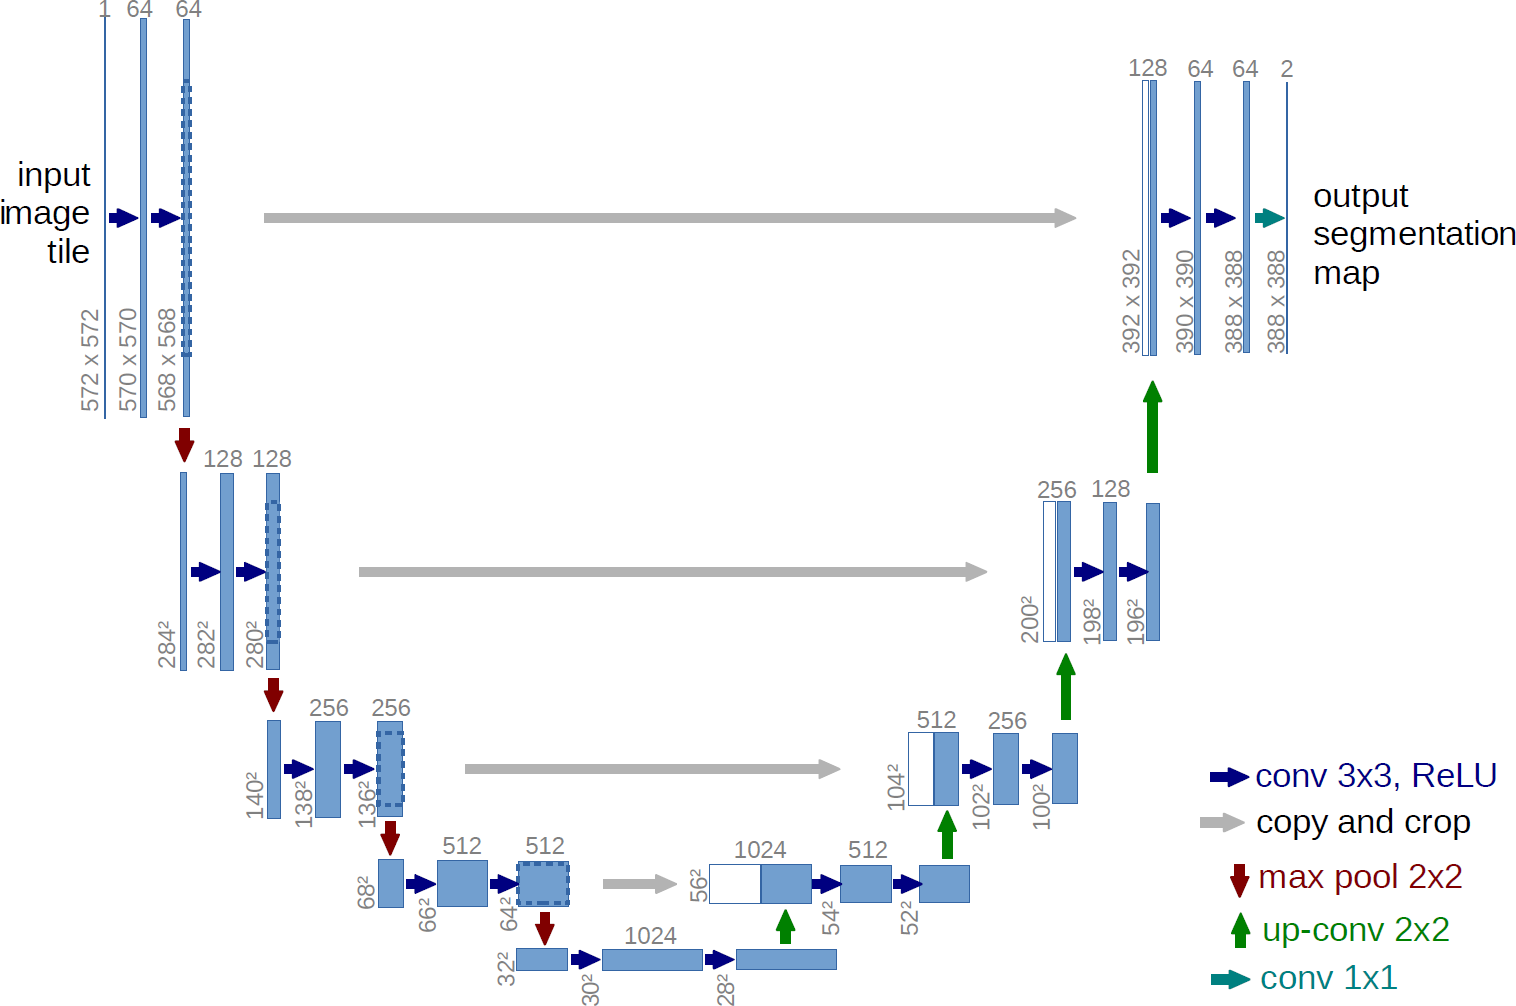
\includegraphics[width=0.9\textwidth]{ronneberger_architecture}
		\caption{Original U-Net architecture first proposed in 2015 by Ronneberger et al. \cite{Ronneberger_2015}. The model consists of symmetric encoding (left) and decoding (right) pathways. Residual skip connections allow for concatenation of extracted image features at different resolutions in order to provide both high-level localisation and high resolution local information for accurate segmentation \cite{Nemoto_2020}. Figure redrawn from Ronneberger et al. \cite{Ronneberger_2015}.}
		\label{fig:unet}
	\end{center}
\end{figure}

\subsection{Activation functions}

Activation functions present in U-Net introduce non-linearity into the model, to enable learning of sophisticated features, beyond those extractable by matrix multiplication alone \cite{Maier2019}. Additionally, ReLU (rectified linear unit) decreases the computational burden compared to typical activation functions (such as tanh and sigmoid), whilst preserving the requirement for non-linearity \cite{Chigozie2018}. However, activation design is an ongoing area of research, with some studies noting performance improvements under modified ReLU functions (i.e. LeakyReLU) \cite{Lin2018}. Additional theory on activation functions is provided in section \ref{sec:act}.

\subsection{Data augmentation}

Pre-processing for U-Net architecture routinely incorporates data augmentation, to add biologically relevant sources of variation to the training data \cite{Maier2019, Hesamian2019, Lundervold2019}. Thus, improving both model robustness and data-use efficiency \cite{Ronneberger_2015}. Dosovitskiy et al. demonstrated improved inference reliability after increasing their effective dataset size via geometric transformations, voxel intensity modulation, as well as blur and noise filters \cite{Dosovitskiy2014}. Data augmentation is also applied to balance the number of infrequent labels in a biased dataset \cite{Maier2019} - such as those in medical imaging, where relatively smaller ROIs occupy a limited volume of the total contour space \cite{Khan2019}. 


\section{Current U-Net architectures}
U-Net implementations and applications vary broadly across the literature - from simplified 2D versions with 3 downsampling layers and 4 x 4 convolutions \cite{Nemoto_2020}, to 3D models that accept full patient volumes as input \cite{Zhu_2018}. A theoretical benefit of volumetric input is that organs may have axial markers that would be absent from 2D images \cite{Hesamian2019}; model inference may benefit from the richer spatial information provided by 3D inputs \cite{Nemoto_2020}. For example, Nikolov et al. presented a 3D U-Net architecture for head and neck segmentation that accepted multiple context slices in addition to the primary input image \cite{Nikolov_2018} - delivering clinically acceptable contours over most datasets, for all but the smallest organs considered \cite{Nikolov_2018}. Alternative 3D implementations report promising results \cite{ Nikolov_2018, Zhu_2018, _i_ek_2016}. However, studies designed to quantify improvement over the simpler 2D architecture have shown limited performance gains \cite{Nemoto_2020}. In contrast, 3D networks require a significantly higher degree of computational resources, which may pose a challenge for clinical implementation \cite{Nemoto_2020}. In general, state-of-the-art 3D networks are trained and deployed via cloud services \cite{Nemoto_2020}; raising important ethical questions for clinics, where data is typically stored on-site with strict security and privacy protocols in place \cite{Nemoto_2020, Lundervold2019}. In addition, modified networks have experimented with feature summation between up-sampling and skip connections; however, concatenation (as in Ronneberger et al \cite{Ronneberger_2015}) has shown consistently better performance \cite{Zhu_2018}.

Nemoto et al. showed that both 2D and 3D U-Net implementations were more effective than commercially available atlas-based auto segmentation tools for delineation of lung regions  \cite{Nemoto_2020}. A total of 232 patients were selected for model training and testing, with all segmentations determined manually by expert observers. In contrast to previous U-Net models mentioned in this review, Nemoto et al. made use of batch normalisation layers (which aim to reduce the effect of bias output distributions from the previous layer to accelerate training \cite{santurkar2018}). Wilcoxon signed-rank testing showed that performance gains over atlas segmentation for both U-Net architectures were statistically significant with $P_{val}<0.01$, and mean DSC improvement of 2.7\% \cite{Nemoto_2020}. However, no statistically significant difference was observed between 2D and 3D U-Net models \cite{Nemoto_2020}, indicating that in the case of lung segmentation (a relatively large structure compared with the model output), the addition of axial input data did not translate to improved contours \cite{Nemoto_2020}.
%
%
\section{State-of-the-art models for bladder and rectum contouring}
Deep-learning segmentation has consistently shown significant improvements over traditional techniques: pixel intensity thresholding, and atlas-based image registration \cite{Cardenas2019}. In the case of pelvic imaging, poor contrast due to similar CT numbers between OARs and high variation in both location and size across patient cohorts restrict the utility of intensity and atlas-based methods \cite{acosta2013}. In addition to this, atlas approaches tend to have reduced performance in the segmentation of small volume organs \cite{acosta2013}. Ayadi et al. conducted a multi-centre prostate cancer study to evaluate the performance of a multi-atlas strategy. Expert contours were compared with Elekta's Atlas-Based Auto-segmentation (ABAS) for 26 patients, resulting in average DSC values of 0.80 $\pm$ 0.19 for the bladder, and 0.66 $\pm$ 0.09 for the rectum - requiring significant manual correction for use in RT \cite{Ayadi2011}.

In comparison, Liu et al. examined the performance of the original U-Net architecture in the segmentation of pelvic OARs. Average DSC scores for CT segmentation of 105 patients were reported as 0.90 $\pm$ 0.11 and 0.78 $\pm$ 0.03 for the bladder and rectum, respectively \cite{Liu_2020}. This is comparatively lower than 2D U-Net results presented by Kazemifar et al. (see Figure \ref{fig:kazemifar_unet} for schematic) who modified the original architecture via batch normalisation, increasing dropout rates, stochastic gradient descent optimisation (SGD) rather than adaptive moment optimisation (Adam), and an additional downsampling block \cite{Kazemifar_2018}. Using a DSC surrogate loss function, excellent agreement was found between observer and model contours for the 85 prostate cancer patients included in the study; with average DSCs of 0.95 $\pm$ 0.04 and 0.92 $\pm$ 0.06 for the bladder and rectum \cite{Kazemifar_2018}. In a follow-up study, Bologapal and Kazemifar et al. attempted 3D U-Net architecture with an additional ResNet block (designed to improve optimisation on extremely deep networks, by minimising numerically unstable gradient flow \cite{Maier2019} i.e. the degradation problem \cite{He2015deep}), in an attempt to further improve bladder and rectum segmentation. Results showed a larger deviation between expert and model contours for the rectum, with a DSC of 0.95 $\pm$ 1.5 and 0.84 $\pm$ 3.7 for bladder and prostate, respectively \cite{Balagopal_2018}. 

\begin{figure}
	\begin{center}
		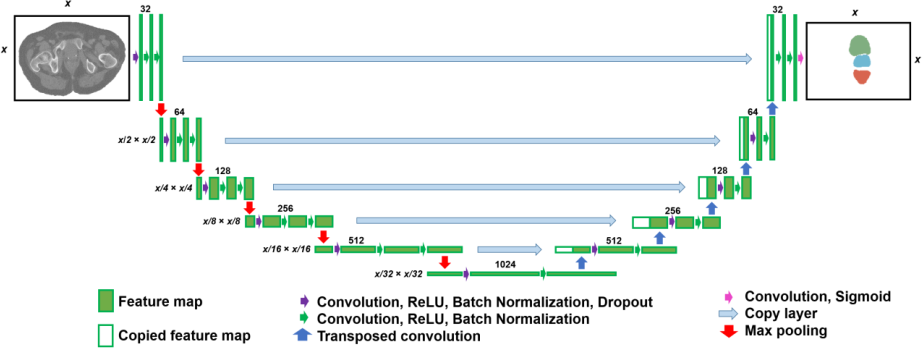
\includegraphics[width=1.05\textwidth]{kazemifar_unet}
		\caption{Modified U-Net architecture used by Kazemifar et al. for state-of-the-art bladder and rectum segmentation in pelvic imaging \cite{Kazemifar_2018}. Addition of batch normalisation layers, increasing dropout rates, and additional downsampling block; when compared to the original U-Net model by Ronneberger et al. Sigmoid activation used as final layer in the network, compared with in-loss function calculation as used in Ronneberger et al. \cite{Ronneberger_2015}. Figure redrawn from Kazemifar et al. \cite{Kazemifar_2018}.}
		\label{fig:kazemifar_unet}
	\end{center}
\end{figure}

Finally, Wong et al. evaluated a commercial deep-learning package (Limbus Contour) based on U-Net architecture and created an independent model for each OAR to be segmented, trained on an average of 328 CT patient scans per model \cite{Wong2020}. Specific details of the architecture are unknown due to the closed nature of the codebase \cite{Wong2020}; however, dropout and batch normalisation were selected during training \cite{Wong2020}. Data augmentation was also used, including image flipping, intensity modulation, and elastic deformations \cite{Wong2020}. Total contouring times for bladder, rectum, femoral heads, prostate, and seminal vesicles were recorded for the deep-learning model and compared to times for a single radiation oncologist (RO). The deep-learning model (DL) showed a significant time improvement (98\% reduction) over manual contouring, with an average inference of 0.4 minutes per patient (excluding manual correction), compared to 21.3 minutes for expert contour (EC) \cite{Wong2020}. In addition, DL accuracy in pelvic OAR contouring was comparable to average IOV measurements between 3 ROs \cite{Wong2020}, highlighting the clinical potential of DL contouring methods in RT. Average worst DSC (lowest DSC score for each patient scan) between DL and EC for the bladder was 0.97, with single worst case 0.95. Average worst EC-EC DSC was measured at 0.96, with single worst 0.94 \cite{Wong2020}. Rectum values showed similar consistency between DL and EC contours, with a DL-EC average worst DSC of 0.78, and single worst of 0.49. EC-EC average worst DSC of 0.79, and single worst of 0.55 \cite{Wong2020}. However, Wong et al. note the study's limitation due to a small patient testing set (20 patients per disease site) \cite{Wong2020} - small datasets are a common challenge in the application of DL methods to segmentation tasks in RT \cite{Ronneberger_2015, Maier2019, Hesamian2019, Lundervold2019}.
%
\section{Class imbalance in medical imaging}
A well-known challenge in applying deep-learning methods to medical image segmentation is the class imbalance between regions-of-interest \cite{Hesamian2019}. In particular, anatomical data in CT imaging often integrates to a much smaller volume than the background voxels, and organs inside this volume vary significantly in size \cite{taghanaki2018}. As a consequence of this input imbalance, the majority of voxels in a segmentation mask may be negatives, resulting in a a biased optimisation strategy that favours negative predictions \cite{taghanaki2018}. Multi-organ segmentation faces the additional challenge of an input class imbalance between organs, leading to parameter updates that are dominated by ROIs with the most voxels in the dataset, as these contribute most significantly to the loss calculation \cite{Khan2019}. Without accounting for this imbalance, the model can quickly become trapped in a local minimum, where optimisation occurs only for the dominant class \cite{Khan2019}. 

Output imbalance refers to a disparity between false-positive and false negative pixels in model predictions. Depending on the context, reducing false-positives may be more important than false-negatives, or vice-versa \cite{taghanaki2018}. For example by placing a higher penalty on false-positives, a model could be tailored to classify less normal tissue as a treatment volume. Conversely, penalising false-negatives may focus optimisation on difficult OARs with poor boundary contrast, reducing under-segmentation \cite{taghanaki2018}.

Studies indicate that the use of class weighting in loss functions can improve results by placing higher importance on contours that infrequently occur in the data, or occupy small anatomical volumes in the patient \cite{taghanaki2018}. Christ et al. showed performance gains by implementing a pixel-frequency class weighting to binary cross-entropy loss, focusing optimisation on difficult regions-of-interest \cite{ferdin2017}; and observed that accurate small lesion segmentation was not possible without class balancing, as their total contribution was less than 1\% of contour voxels \cite{ferdin2017}. In contrast, Taghanaki et al. used weighting and a combination DSC + BCE loss to enforce a desired trade-off between either false-positives or false-negatives (depending on model requirements) to correct for output imbalance; reporting improved DSC scores and lower false-negative rates for multi-organ segmentation across a range of imaging modalities \cite{taghanaki2018}.

